\chapterauthor{Author Name}{Vinicius Francisco da Silva}
\chapter{Conceitos básicos}


\section{Introdução}\label{intro}

\section{Definição}\label{intro}
De maneira bem simples, um compilador é um programa de computador que recebe um arquivo de entrada denominado “programa fonte” realiza uma série de análises e caso haja sucesso em todas as análises é gerado um outro arquivo correspondente denominado “programa alvo”, caso contrário é gerado erro.

\begin{figure}
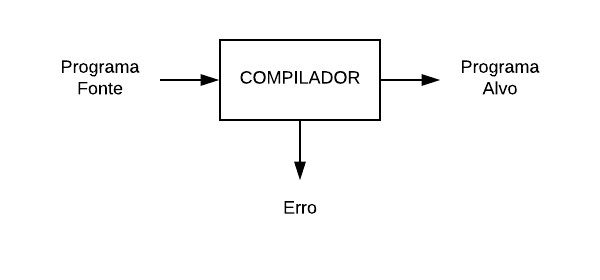
\includegraphics[width=250pt, height=100pt]{chapters/chapter1/figures/imagem1.png}
%%\centerline{\epsfig{/Chapters/chapter1/figures/cat.eps,width=.8\textheight,height=.4\textwidth}}
\caption[List of figure caption goes here]{Figure caption goes here.}
\end{figure}

\subsection{Programa fonte:} 
O programa fonte são arquivos escritos na linguagem de programação x, que será compilador em um compilador próprio para a linguagem x.\\

Todos os elementos  da linguagem presentes no código fonte são denominados “símbolos” que são elementos únicos e indivisíveis. Qualquer outro símbolo que não pertence a linguagem é considerado inválido. Estes símbolos fazem parte do alfabeto (Sigma) da linguagem, na \textbf{imagem 2}  temos o exemplo de um conjunto de símbolos (Alfabeto) da linguagem C.\\



IMAGEM 2\\ \\

O alfabeto $\Sigma$ é um conjunto de n símbolos de uma linguagem x. Este conjunto de símbolos possuí todos os elementos válidos da linguagem, ou seja, aquilo que a linguagem permite está presente neste conjunto.\\

Para reforçar os símbolos são elementos indivisíveis da linguagem, que fazem parte do conjunto denominado alfabeto, representado por $\Sigma$. Fazendo uma analogia, um símbolo da linguagem de programação é como uma letra de uma linguagem comum que falamos, que fazem parte do alfabeto.\\

Na implementação do compilador, os símbolos da linguagem são estruturas que possuem uma série de informações como: lexema, token, classe, endereço, padrão de formação e descrição.\\

IMAGEM 3\\ \\

Nesta sessão serão definidos os lexemas, tokens, padrão de formação e descrição. As classes e os endereços serão abordados nos CAPÍTULOS 7 E 8. \\

\subsubsection{Token}
Um token é um elemento do alfabeto $\Sigma$. Pode-se dizer que um token é um valor correspondente ao símbolo pertencente ao alfabeto. Representa uma unidade léxica. \\

IMAGEM 4\\ \\

\subsubsection{Lexema}
Um lexema é definido com as formas que um token pode ser escrito na linguagem. Tome o identificador como exemplo (id). O token do símbolo é id, porém o id pode ser escrito (nomeado) de várias formas diferentes. Estas formas são considerados os lexemas válidos para o token id. Um outro exemplo é o token constante, que pode ser representado por números na faixa de $-\infty$ á $+\infty$. Estas representações são os lexemas do token constante.\\

Dentre os símbolos do alfabeto o único que não é utilizado é o espaço em branço, está presente no alfabeto da linguagem mas não possui importância para a análise do compilador, sendo descartado nas primeiras fases do compilador. Pode-se considerar o espaço em branco apenas como um delimitador léxico.\\

IMAGEM 5\\ \\

\subsubsection{Padrão de formação de lexema}
É uma expressão regular que define a formação dos  lexemas de um token.\\

Exemplos na linguagem Pascal:\\

\begin{table}[!h]%1
%\noautomaticrules
\tabletitle{Now we are engaged $(a_g^a)$ $\big(a_g^a\big)$ in a great civil war, testing whether that
nation, or any nation so conceived.}%
\begin{tabular}{|c|c|c|}

\textbf{Token} & \textbf{Lexema} & \textbf{Padrão de formação} \\
\hline
constante & 0,-2,20,... & (-digito+ $\cup$ digito+)   \\
\hline
\textless & \textless & \textless\\
\hline
if   & If,IF,if,iF & (i $\cup$ I)(f $\cup$ F)\\
\hline
constante & "a", "String", "cadeia de caracteres" & "(Símbolos de $\Sigma$)"\\
\hline
while & While,WHILE,while & (W $\cup$ w)(h $\cup$ H)(i $\cup$ I)(l $\cup$ L)(e $\cup$ E)\\
\end{tabular}
\end{table}


\subsubsection{Descrição do símbolo} 
A descrição de símbolos é uma rotulação feita para identificar os símbolos em uma linguagem de programação. Na implementação do compilador esta informação não é utilizada, porém ela é de extrema importância para a separação e identificação dos símbolos da linguagem.\\

Estes rótulos são:

\begin{itemize}
\item Identificadores
\item Constantes numéricas
\item Constantes literais
\item Palavras Reservadas
\item Operador relacional
\end{itemize}

Exemplos:\\

\begin{table}[!h]%1
%\noautomaticrules
\tabletitle{Now we are engaged $(a_g^a)$ $\big(a_g^a\big)$ in a great civil war, testing whether that
nation, or any nation so conceived.}%
\begin{tabular}{|c|c|c|c|}

\textbf{Token} & \textbf{Lexema} & \textbf{Padrão de formação} & \textbf{Descrição} \\
\hline
constante & 0,-2,20,... & (-digito+ $\cup$ digito+) & Constante numérica \\
\hline
constante & "Cadeia de caracteres", ... & ("Símbolos de $\Sigma$")* & Constante literal\\
\hline
for & For, for, FOR, … & (f $\cup$ F)(o $\cup$ O)(r $\cup$ R) & Palavra reservada\\
\hline
identificador & a,ab,n,x, … & ($_ \cup$ d)($_ \cup$ d $\cup$ l)* & Identificador\\
\hline
if & if,If,IF & (i $\cup$ I)(f $\cup$ F) & Palavra reservada\\
\end{tabular}
\end{table}

\subsection{Programa alvo}
É um programa gerado pelo compilador, correspondente ao programa passado na entrada como mostra a \textbf{Figura 1}. Pode-se dizer que em quase todos os compiladores que o programa alvo é um programa Assembly de uma máquina específica.\\

IMAGEM 5\\

\section{Estrutura}

O compilador é dividivo em duas partes: A análise e a síntese.

\begin{figure}
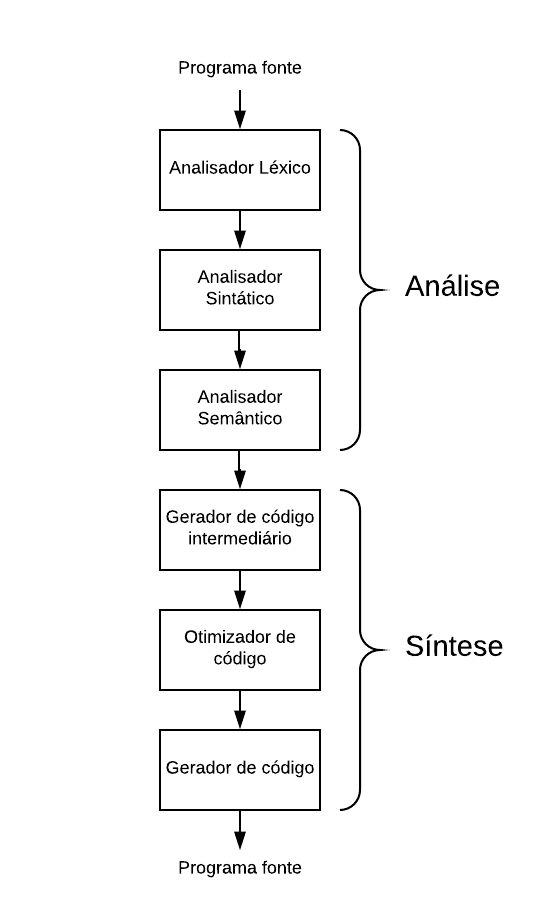
\includegraphics[width=337pt, height=320pt]{chapters/chapter1/figures/imagem6.png}
%%\centerline{\epsfig{/Chapters/chapter1/figures/cat.eps,width=.8\textheight,height=.4\textwidth}}
\caption[List of figure caption goes here]{Figure caption goes here.}
\end{figure}

\subsection{Análise}
É a parte que o compilador recebe o programa fonte e faz uma série de análises léxicas, sintáticas, e semânticas. É através da análise que caso o código fonte tenha erro o mesmo é gerado e tratado. É uma etapa que certifica que o arquivo fonte recebido na entrada está pronto para ser “tranformado” em código alvo.\\

A etapa de análise é dividida em 3: Analisador Léxico, Analisador Sintático, Analisador Semântico. \\

\subsubsection{Analisador Léxico}
Responsável por percorrer o código fonte realizando a identificação dos lexemas (ação semântica) e o atribuindo a um símbolo com seu token correspondente. É através do analisador léxico que comentários, espaços em branco são descartados. \\

IMAGEM 7\\

Fazendo uma alusão, podemos dizer que o processo do analisador léxico é como o processo de verificação de palavras em um texto, frase, poema, etc …\\

Vemos o exemplo abaixo, utilizando a linguagem de programação C e a língua portuguesa.


IMAGEM 7 E 8\\

\subsubsection{Analisador Sintático} 
É responsável por agrupar os tokens dos símbolos em estruturas hierárquicas. \\ 

Esta estrutura hierárquica denominado árvore de parse é fruto da derivação de uma gramática livre de contexto. Este processo de agrupamento tem a função de realizar a análise gramatical que é simplesmente conferir o que foi escrito no programa fonte com o que está na gramática da linguagem. \\

Fazendo alusão podemos dizer que o agrupamento de tokens na análise sintática é um agrupamento de palavras na linguagem falada. Não é possível verificar a coerência gramatical com apenas uma palavra. É necessário agrupar os elementos para que esta analise seja feita. \\

Tome parte de uma gramática livre de contexto GLC abaixo e parte da gramática da língua portuguesa. \\

\begin{center}
Linguagem C
\end{center}

G:\\ \\
\textbf{S} → int \textbf{Atribuicao} $|$ char \textbf{Atribuicao} $|$ byte \textbf{Atribuicao}\\
\textbf{Atribuicao} → id = \textbf{Valores};\\
\textbf{Valores} → const $|$ id \\ \\ \\

\begin{center}
Língua Portuguesa
\end{center}

G:\\ \\
\textbf{Oracao} → \textbf{Sujeito} \textbf{Predicado} \\
\textbf{Sujeito} → artigo substantivo \\
\textbf{Predicado} → \textbf{VerboLigativo} \textbf{PredicativoSujeito} \\
\textbf{VerboLigativo} → verbo \\
\textbf{PredicativoSujeito} → adjetivo
